\documentclass[../main.tex]{subfiles}

\usepackage{amsmath}
\usepackage{amssymb}

\begin{document}

\subsection{Leveraging Citation Networks for Medical TAR}

Systematic reviews utilise research evidence to provide clinical practice recommendations. The communication of medical research follows standardised formatting conventions and primarily occurs through peer-reviewed publication \cite{BMCMedicalResearch}. When authors compose research papers, they must reference related works to substantiate their claims and situate their findings within the existing body of knowledge. These citations follow standardised formatting guidelines and are documented in the paper's reference section. This rigorous documentation of citations enables analysis of the relationships between research papers, operating under the assumption that studies that cite or are cited by a research article are relevant to that research.

\subsubsection{Relation analysis improves CAL TAR performance}

Recent advances in medical CAL TAR have indirectly demonstrated the benefit of relationship analysis for citations. The current leading encoder model, $BioLinkBERT_{base}$ achieved state-of-the-art performance on the CLEF dataset in a CAL setting by leveraging citations networks between research papers \cite{yasunaga2022linkbertpretraininglanguagemodels, goharian_reproducibility_2024}. 


The $LinkBERT$ approach was to view a pertaining corpus as a graph of documents, with each document being a vertex and hyperlinks forming edges between documents. These related documents were then placed within the same context window. The approach differs from traditional $BERT$ architectures, which randomly allocate documents to context windows without considering their relationships. While this might appear similar to curriculum learning approachings, $LinkBERT$ is distinct in that it does not organise context windows by difficulty level. 

$BioLinkBERT$, a domain-specific adaption of $LinkBERT$, was developed specifically for biomedical aplications and pretrained exclusively on PubMed articles, using citation relationships to estimate document relationships \footnote{https://huggingface.co/michiyasunaga/BioLinkBERT-base}. The model trianing process incorporated standard masked language modelling and next-sentence prediction techniques. Analysis of both the base model (100M parameters) and large model (340M parameters) against $PubMedBERT$ across multiple benchmarks:  BLURB\cite{guDomainSpecificLanguageModel2021}, MedQA-USMLE\cite{jinWhatDiseaseDoes2020}, and MMLU-professional medicine\cite{hendrycksMeasuringMassiveMultitask2021}. The results demonstrated $BioLinkBERT_{large}$'s superior performance across all evaluated benchmarks, notably achieving a 3.2\% improvement over PubMedBERT in the BLURB score.


\begin{figure}[t]
    \centering
    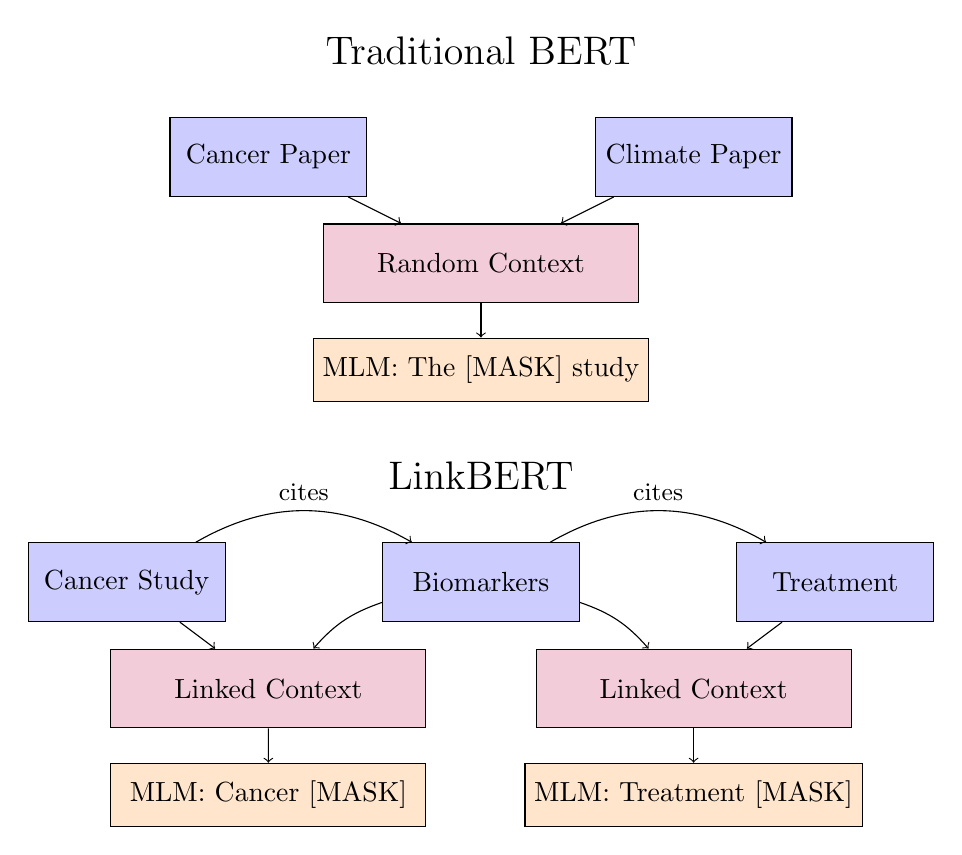
\begin{tikzpicture}[
        doc/.style={rectangle, draw, fill=blue!20, minimum width=2.5cm, minimum height=1cm},
        window/.style={rectangle, draw, fill=purple!20, minimum width=4cm, minimum height=1cm},
        mlm/.style={rectangle, draw, fill=orange!20, minimum width=4cm, minimum height=0.8cm},
        node distance=2cm,
        scale=0.9
    ]
    % Traditional BERT (top)
    \node[align=center] at (-3,5) {\Large Traditional BERT};
    \node[doc] (a1) at (-6,3.5) {Cancer Paper};
    \node[doc] (a2) at (0,3.5) {Climate Paper};
    \node[window] (b1) at (-3,2) {Random Context};
    \node[mlm] (m1) at (-3,0.5) {MLM: The [MASK] study};
    
    \draw[->] (a1) -- (b1);
    \draw[->] (a2) -- (b1);
    \draw[->] (b1) -- (m1);
    
    % LinkBERT (bottom) - with increased horizontal spacing
    \node[align=center] at (-3,-1) {\Large LinkBERT};
    \node[doc] (c1) at (-8,-2.5) {Cancer Study};
    \node[doc] (c2) at (-3,-2.5) {Biomarkers};
    \node[doc] (c3) at (2,-2.5) {Treatment};
    
    \node[window] (d1) at (-6,-4) {Linked Context};
    \node[mlm] (n1) at (-6,-5.5) {MLM: Cancer [MASK]};
    
    \node[window] (d2) at (0,-4) {Linked Context};
    \node[mlm] (n2) at (0,-5.5) {MLM: Treatment [MASK]};
    
    % Citations with curved arrows
    \draw[->, bend angle=30] (c1) to[bend left] node[midway,above] {\small cites} (c2);
    \draw[->, bend angle=30] (c2) to[bend left] node[midway,above] {\small cites} (c3);
    
    % Context connections with slight bends to avoid overlap
    \draw[->] (c1) -- (d1);
    \draw[->] (c2) to[bend right=15] (d1);
    \draw[->] (c2) to[bend left=15] (d2);
    \draw[->] (c3) -- (d2);
    \draw[->] (d1) -- (n1);
    \draw[->] (d2) -- (n2);
    
    \end{tikzpicture}
    \caption{Comparison of document processing in traditional BERT versus LinkBERT. Traditional BERT (top) randomly groups documents into context windows, while LinkBERT (bottom) uses citation relationships to create meaningful document groupings for pretraining. The citation-based grouping ensures that semantically related documents are processed together during masked language modeling tasks.}
    \label{fig:linkbert-comparison}
\end{figure}


Current research on document relationship-based encoders in the CAL process has not definitively established that document relations are the primary driver of performance improvements. Furthermore, the assumption that larger models consistently yield better results is not always the case. The author replicated the previously reported Goldilock Reproduce study, where $BioLinkBERT_{base}$ formed the classifier, except changing the model to the $BioBERT_{large}$ variant\footnote{https://huggingface.co/michiyasunaga/BioLinkBERT-large} as a classifier model, yet only achieved higher performance in R-Precision in 7 of 12 datasets/policy combinations.  The empirical results, detailed in Table \ref{tab:results-average}, show peak R-precision values of 0.847 for the relevancy selection policy (at FPT epoch 2) and 0.832 for uncertainty selection (at FPT epoch 1).Statistical analysis using the Friedman test revealed significant differences between Further Pre-Training (FPT) epochs in only 4 of 12 datasets when examined individually. More importantly, when analyzing all datasets collectively, no statistically significant differences emerged in R-precision values across FPT epochs for either relevancy selection or uncertainty selection policies. This findiing challenges the previously documented  ``Goldilocks problem'' observed in non-medical domains. Specifically demonstrating that FPT does not yield statistically significant improvemnts in R-Precision. 

This replication study has generated valuable insights for this PhD investigation. A significant finding indicates that seeking an optimal pretraining epoch within the CLEF dataset is unlikely to be productive for future research endeavors. The experimental design revealed several methodological considerations, particularly regarding the implementation of hyperparameters without robust empirical justification. These include the selection of a batch size of 25, the decision to fine-tune for 20 epochs, and the termination criterion of 501 labeled documents. These parameter choices, while functional, may impose limitations on potential improvements to encoder CAL process performance within the experimental framework.

The significance of these limitations becomes particularly evident when considering that observed R-Precision values approach the theoretical maximum of 1.0, with some instances achieving values as high as 0.945. In the context of the Goldilocks reproduce paper, datasets showing lower performance metrics, such as the CLEF 2019 dataset (with R-precision values of 0.82 for relevancy and 0.791 for uncertainty), present additional analytical challenges. The utilization of Large Language Models (LLMs) introduces complexity in interpreting the underlying causes of reduced performance in these cases.

While exploring larger, more sophisticated models presents a potential avenue for improvement, this approach faces practical constraints. Given the limitations of High-Performance Computing resources and PhD time constraints, pursuing research dependent on the development and availability of superior LLMs may not be the most pragmatic direction.

A crucial observation emerged from this research regarding the relationship between early document classification and overall performance. In iterations where strong performance was ultimately achieved at iteration 20, a notably higher number of relevant documents were classified earlier in the CAL process. This finding aligns with theoretical expectations: a larger corpus of correctly classified documents early in the process provides a more robust foundation for subsequent classification decisions. This insight carries significant implications for the next phase of this PhD research, suggesting that enhancing document availability in the early stages of the active learning process could substantially improve overall performance outcomes.

While $BioLinkBERT$ represents a sophisticated approach that combines citation networks with contextual language understanding, this integration presents both advantages and limitations. The model's ability to capture complex semantic relationships between documents is valuable, but the contextual processing introduces potential inefficiencies. During pretraining, when linked documents are placed in the same context, the model must process all content within those documents—including sections that may be tangential or unrelated to the citing paper's specific reference. This contextual noise could potentially dilute the precision of the more direct relationships that citations inherently represent. In contrast, pure citation links directly capture intentional scholarly connections made by domain experts, providing a cleaner signal without the additional complexity of processing potentially irrelevant contextual information.

A fundamental question emerges from this research: Is contextual understanding of references truly necessary for effective CAL? Several factors suggest that citation networks alone might be sufficient and potentially superior. First, citations themselves represent a form of knowledge distillation, where domain experts have already identified meaningful relationships between documents. Second, analysing reference networks is computationally more efficient than processing full textual contexts. Third, citation network models tend to be more stable when updated, compared to contextual models. Fourth, the contextualization of citation networks may actually introduce noise into what would otherwise be clear citation signals.


\begin{table}[htbp]
    \centering
    \footnotesize
    \setlength{\tabcolsep}{4pt}
    \begin{tabular}{l>{\raggedright\arraybackslash}p{1.2cm}ccccc}
    \hline
    \textbf{Collection} & \textbf{Dataset size} & \textbf{Model} & \multicolumn{2}{c}{\textbf{R-Precision (↑)}} & \multicolumn{2}{c}{\textbf{Friedman (p)}} \\
    \cline{4-7}
    & & & \textbf{Rel.} & \textbf{Unc.} & \textbf{Rel.} & \textbf{Unc.} \\
    \hline
    \multirow{6}{*}{\makecell[l]{Clef 2019\\dta test}} & 
    \multirow{6}{*}{8} & BiolinkBert-Base-ep0 & \textbf{0.909} & \textbf{0.857} & \multicolumn{2}{c}{---} \\
    & & BiolinkBert-Large-ep0 & 0.897 & 0.803 & \multirow{5}{*}{0.914} & \multirow{5}{*}{0.632} \\
    & & BiolinkBert-Large-ep1 & 0.827 & 0.832 & & \\
    & & BiolinkBert-Large-ep2 & 0.812 & 0.774 & & \\
    & & BiolinkBert-Large-ep5 & 0.841 & 0.814 & & \\
    & & BiolinkBert-Large-ep10 & 0.881 & 0.846 & & \\
    \hline
    \multirow{6}{*}{\makecell[l]{Clef 2017\\test}} & 
    \multirow{6}{*}{30} & BiolinkBert-Base-ep0 & 0.812 & 0.794 & \multicolumn{2}{c}{---} \\
    & & BiolinkBert-Large-ep0 & 0.828 & 0.797 & \multirow{5}{*}{\textbf{\textless0.05}} & \multirow{5}{*}{\textbf{\textless0.05}} \\
    & & BiolinkBert-Large-ep1 & 0.826 & \textbf{0.827} & & \\
    & & BiolinkBert-Large-ep2 & \textbf{0.858} & 0.804 & & \\
    & & BiolinkBert-Large-ep5 & 0.827 & 0.777 & & \\
    & & BiolinkBert-Large-ep10 & 0.799 & 0.757 & & \\
    \hline
    \multirow{6}{*}{\makecell[l]{Clef 2017\\train}} & 
    \multirow{6}{*}{20} & BiolinkBert-Base-ep0 & \textbf{0.838} & 0.761 & \multicolumn{2}{c}{---} \\
    & & BiolinkBert-Large-ep0 & 0.778 & 0.765 & \multirow{5}{*}{\textbf{\textless0.05}} & \multirow{5}{*}{0.28} \\
    & & BiolinkBert-Large-ep1 & 0.808 & 0.789 & & \\
    & & BiolinkBert-Large-ep2 & 0.767 & 0.701 & & \\
    & & BiolinkBert-Large-ep5 & 0.816 & 0.786 & & \\
    & & BiolinkBert-Large-ep10 & 0.827 & \textbf{0.796} & & \\
    \hline
    \multirow{6}{*}{\makecell[l]{Clef 2018\\test}} & 
    \multirow{6}{*}{30} & BiolinkBert-Base-ep0 & 0.794 & 0.780 & \multicolumn{2}{c}{---} \\
    & & BiolinkBert-Large-ep0 & 0.789 & 0.774 & \multirow{5}{*}{0.52} & \multirow{5}{*}{0.50} \\
    & & BiolinkBert-Large-ep1 & \textbf{0.812} & 0.790 & & \\
    & & BiolinkBert-Large-ep2 & 0.797 & \textbf{0.791} & & \\
    & & BiolinkBert-Large-ep5 & 0.763 & 0.773 & & \\
    & & BiolinkBert-Large-ep10 & 0.763 & 0.769 & & \\
    \hline
    \multirow{6}{*}{\makecell[l]{Clef 2019\\DTA int.\\train}} & 
    \multirow{6}{*}{20} & BiolinkBert-Base-ep0 & 0.939 & 0.923 & \multicolumn{2}{c}{---} \\
    & & BiolinkBert-Large-ep0 & 0.939 & 0.902 & \multirow{5}{*}{0.78} & \multirow{5}{*}{0.50} \\
    & & BiolinkBert-Large-ep1 & 0.941 & 0.935 & & \\
    & & BiolinkBert-Large-ep2 & 0.948 & 0.921 & & \\
    & & BiolinkBert-Large-ep5 & 0.952 & 0.945 & & \\
    & & BiolinkBert-Large-ep10 & \textbf{0.945} & \textbf{0.947} & & \\
    \hline
    \multirow{6}{*}{\makecell[l]{Clef 2019\\DTA int.\\test}} & 
    \multirow{6}{*}{20} & BiolinkBert-Base-ep0 & \textbf{0.934} & \textbf{0.900} & \multicolumn{2}{c}{---} \\
    & & BiolinkBert-Large-ep0 & 0.899 & 0.856 & \multirow{5}{*}{0.87} & \multirow{5}{*}{\textbf{\textless0.05}} \\
    & & BiolinkBert-Large-ep1 & 0.904 & 0.840 & & \\
    & & BiolinkBert-Large-ep2 & 0.909 & 0.878 & & \\
    & & BiolinkBert-Large-ep5 & 0.882 & 0.835 & & \\
    & & BiolinkBert-Large-ep10 & 0.865 & 0.841 & & \\
    \hline
   
    \end{tabular}
    \caption{Performance comparison across different collections and models}
    \label{tab:results}
\end{table}

\begin{table}[htbp]
    \centering
    \caption{Average R-precision of each FPT epoch for CLEF dataset}
    \begin{tabular}{l>{\raggedright\arraybackslash}p{1.2cm}ccccc}
        \textbf{Policy} & \textbf{ep0} & \textbf{ep1} & \textbf{ep2} & \textbf{ep5} & \textbf{ep10} \\
        \hline
        Uncertainty & 0.813 & 0.832 & 0.813 & 0.815 & 0.814 \\
        Relevancy & 0.840 & 0.845 & 0.847 & 0.842 & 0.835 \\
    \hline

    \end{tabular}
    \label{tab:results-average}
\end{table}



\subsubsection{Direct citation network mining within medicine research}

Performant, simple, and robust approaches to citation network mining already exist within medicial research. Let G be a citation graph where:

\begin{itemize}
    \item $D_i$ represents a research article of interest as a vertex in G
    \item $D_{ip}$ represents the set of articles referenced by $D_i$
    \item $D_{if}$ represents the set of articles that reference $D_i$
    \item Both sets are subsets of G: $D_{ip}, D_{if} \subset G$
    \item $D_{ip} \cap D_{if} = \emptyset$, so searching both sets will provide different relevant articles
\end{itemize}

Relevancy is defined as a function $R: D \rightarrow [0,1]$, where:

\begin{itemize}
    \item 0 denotes no relevance
    \item 1 denotes maximum relevance
    \item For any set of documents $D_{set}$, relevancy is defined as $R(D_{set}) = {R(d) | d \in D_{set}}$
\end{itemize}

Two primary citation network mining approaches are defined:
\begin{itemize}
    \item Backward citation searching (BCS): examining all articles in $D_{ip}$\cite{lefebvre2011cochrane, akers2009systematic}
    \item Forward citation searching (FCS): examining all articles in $D_{if}$*\footnote{FCS involves using a citation index to identify studies that cite a source study. A citation index is a database of scholarly articles and their citations, such as PubMed, Google Scholar, Scopus or OpenAlex}
\end{itemize}

Backward and forward citation searching (BCS and FCS) are both straightforward and effective approaches that inherently respect the chronological relationships between research articles, as papers can only cite previously published work. The significance of these methods is demonstrated by their recommended use in Cochrane systematic reviews, particularly during the identification phase. A study of Cochrane reviews conducted between November 2016 and January 2017 found that 87\% reported using BCS, while 9\% utilized FCS \cite{briscoeConductReportingCitation2019}.. The Cochrane Handbook explicitly mandates the use of BCS (criterion C30) in the search stage, though it makes no mention of FCS  \cite{MECIRManualCochrane}. However, neither the use of BCS nor FCS is addressed in the Handbook's guidelines for the screening phase.


The application of Backward and Forward Citation Searching (BCS and FCS) within an active learning process represents an understudied area of research (see Figure \ref{fig:search-results} for search strategy details). To establish the novelty of this augmentation, several key distinctions must be clarified. While this PhD research focuses on the title and abstract screening phase of systematic review generation, BCS and FCS have traditionally been confined to the identification phase (as illustrated in Figure \ref{fig:selection_and_screening}). Conventionally, title and abstract screening serves to reduce the workload for the more resource-intensive full-text screening phase. However, from a computational perspective, restricting the screening process to titles and abstracts is unnecessary, as the computational cost remains manageable when including full texts.
 
\begin{figure}[htbp]
    \centering
    \begin{tikzpicture}[
        node distance = 0.5cm,
        box/.style={rectangle, draw, text width=4cm, minimum height=1cm, align=center},
        query/.style={rectangle, draw, fill=gray!10, text width=4cm, minimum height=2.5cm, align=center}
    ]
        % Search queries side by side
        \node[query] (q1) {Search Query 1:\\
            (``backward citation'' OR\\``citation analysis'')\\
            AND ``active learning''};
        \node[query] (q2) [right=0.5cm of q1] {Search Query 2:\\
            (``citation graph'' OR\\``citation network'') AND\\(``active learning'' OR\\``interactive learning'')};
        \node[query] (q3) [right=0.5cm of q2] {Search Query 3:\\
            (``bibliometric analysis'' OR\\``reference mining'') AND\\(``selective sampling'' OR\\``query learning'')};
            
        % Results box below
        \node[box] (results) [below=1cm of q2] {No Related Documents Found};
            
        % Arrows
        \draw[-stealth] (q1) -- (results);
        \draw[-stealth] (q2) -- (results);
        \draw[-stealth] (q3) -- (results);
        
    \end{tikzpicture}
    \caption{Results from literature search on citation index arxiv and pubmed demonstrating absence of related works, ran on 13th November 2024}
    \label{fig:search-results}
\end{figure}
\begin{center}
\begin{tikzpicture}[
    > = {Stealth[scale=1.2]},
    vertex/.style = {circle, draw, minimum size=1.2cm, inner sep=1pt},
    ref_edge/.style = {->, thick, blue},
    label_style/.style = {font=\small}
]

% Main document Di
\node[vertex, fill=yellow!20] (Di) at (0,0) {$D_i$};

% Past references (Dip) - More fanned out
\node[vertex] (Dip1) at (-3,2.5) {$D_{ip1}$};
\node[vertex] (Dip2) at (0,3) {$D_{ip2}$};
\node[vertex] (Dip3) at (3,2.5) {$D_{ip3}$};

% Future references (Dif) - More fanned out
\node[vertex] (Dif1) at (-3,-2.5) {$D_{if1}$};
\node[vertex] (Dif2) at (0,-3) {$D_{if2}$};
\node[vertex] (Dif3) at (3,-2.5) {$D_{if3}$};

% Edges for past references
\draw[ref_edge] (Di) -- (Dip1);
\draw[ref_edge] (Di) -- (Dip2);
\draw[ref_edge] (Di) -- (Dip3);

% Edges for future references
\draw[ref_edge] (Dif1) -- (Di);
\draw[ref_edge] (Dif2) -- (Di);
\draw[ref_edge] (Dif3) -- (Di);

% Labels for sets
% \node[label_style] at (-4,2) {$D_{ip}$ (Referenced by $D_i$)};
% \node[label_style] at (-4,-2) {$D_{if}$ (References to $D_i$)};

% Relevancy function examples
\node[label_style] at (5,2.5) {$R(D_{ip1}) = 1$};
\node[label_style] at (5,2) {$R(D_{ip2}) = 1$};
\node[label_style] at (5,1.5) {$R(D_{ip3}) = 0$};
\node[label_style] at (5,-1.5) {$R(D_{if1}) = 1$};
\node[label_style] at (5,-2) {$R(D_{if2}) = 0$};
\node[label_style] at (5,-2.5) {$R(D_{if3}) = 0$};

% Time arrow (vertical)
\draw[{Stealth[scale=1.5]}->, thick] (7,3.5) -- (7,-3.5);
\node[label_style] at (7,3.8) {Past};
\node[label_style] at (7,-3.8) {Future};

\end{tikzpicture}
\end{center}

These citation networks are rich in relevant documents, much more so than that of the document collection, which is demonstrated by the author comparing precision of pools using BCS and FCS against that of the entire document collection in Figure \ref{fig:citation-network-mining}. The logical, and simple augmentation of the encoder CAL approach would be to exhaust both BCS and FCS networks of a seed document prior to initiating the encoder CAL process. 

The theoretical benefits of citation network mining are that it can be used to augment the CAL process in ways that overcome some of the limitations of this process.  Firstly, CAL requires labelled data to train a classifier model, which is assumed to perform better with more data points. Encoder CAL approaches suffer disproportionately to that of feature-based CAL approaches due to their need for larger amounts of training data to effectively learn meaningful representations. This is because encoder models like BERT need to learn complex contextual relationships between words and concepts, whereas feature-based models can rely on simpler statistical patterns. When working with limited labeled data in the early stages of screening, encoder models may struggle to generalise well, potentially leading to suboptimal performance in identifying relevant documents. As discussed in the Encoder CAL process, often a single sample seed document is used during the first epoch for fine-tuning. A better approach would be to exhaust the citation network of that seed document first for labelling, before using revealed relevant documents to fine-tune the model, potentially resulting in a more performant model at the earlier stages of screening with less oracle cost. 

\subsubsection{Extending current citation network mining approaches}

BCS and FCS citation network mining faces a significant limitation in its inability to identify indirect citation relationships. An indirect citation occurs when research papers are connected through intermediate references, forming a chain of citations rather than a direct reference. For instance, when document $D_i$ cites document $D_{ip1}$, which in turn cites document $D_{ip2}$, a relationship exists between $D_i$ and $D_{ip2}$ despite the absence of a direct citation. This relationship represents an indirect citation, which is shown in Figure \ref{fig:indirect-citation}. This causes issues if $D_{ip1}$ is not included in the document pool, as $D_i$ and $D_{ip2}$ will no longer have an edge. 

This constraint makes it unsuitable as a complete solution for document relationship discovery for the encoder CAL process. However, researchers have proposed several modifications to the citation network mining process to address this limitation:

\begin{center}
    \begin{tikzpicture}[
        > = {Stealth[scale=1.2]},
        vertex/.style = {circle, draw, minimum size=1.2cm, inner sep=1pt},
        ref_edge/.style = {->, thick, blue},
        indirect_edge/.style = {->, thick, red, dashed},
        label_style/.style = {font=\small}
    ]
    
    % Main document Di
    \node[vertex, fill=yellow!20] (Di) at (0,0) {$D_i$};
    
    % Direct reference
    \node[vertex] (Dip1) at (-2,2) {$D_{ip1}$};
    
    % Indirect reference
    \node[vertex] (Dip2) at (2,4) {$D_{ip2}$};
    
    % Add edges
    \draw[ref_edge] (Di) -- (Dip1) node[midway, left] {Direct};
    \draw[ref_edge] (Dip1) -- (Dip2) node[midway, right] {Direct};
    \draw[indirect_edge] (Di) to[bend right] node[midway, right] {Indirect} (Dip2);
    
    % Time arrow (vertical)
    \draw[{Stealth[scale=1.5]}->, thick] (4,4.5) -- (4,-1);
    \node[label_style] at (4,4.8) {Past};
    \node[label_style] at (4,-1.3) {Future};
    
    % Legend
    \node[label_style] at (6,2) {Legend:};
    \draw[ref_edge] (5,1.5) -- (7,1.5) node[right] {Direct citation};
    \draw[indirect_edge] (5,1) -- (7,1) node[right] {Indirect citation};

    \end{tikzpicture}

    \label{fig:indirect-citation}
    \end{center}


\begin{itemize}
    \item \textbf{Matching isolated nodes based on similarity metric of their embeddings}: If $N$ is all the documents in the total pool, and $N_{isolated}$ is the set of documents that are not cited by any other document in $N$, then for each document $D_{ip} \in N_{isolated}$, find the document $D_i \in N$ with the highest similarity metric (i.e. cosine similarity) to $D_{ip}$. Add a artificial edge between $D_i$ and $D_{ip}$.
    \item \textbf{Matching isolated compoments on similarity metric of their embeddings}: When analyzing document clusters, some small groups of documents (called isolated components) may be disconnected from the main cluster. These isolated components have fewer connections to other documents, which can reduce classification accuracy. To fix this:
    \begin{itemize}
        \item Identify isolated components $C_{isolated}$ that have fewer or equal nodes than the main cluster
        \item For each node in these isolated components
        \item Calculate a similarity metric (i.e. cosine similarity) to nodes in larger clusters $C_i$
        \item Connect it to the most similar large cluster by adding a artificial edge
    \end{itemize}

\end{itemize}

This constraint however doesn't make it unsuitable as a partial improvement to the encoder CAL process for identifying relevant documents based on the initial seed document. Even without considering indirect citations, assessing the citation network of the seed document is potentially more relevant than that of the entire document collection. In table \ref{tab:citation-network-mining} it is unequivacle that the precision of relevant documents within pools using BCS, FCS  and both together against that of the entire document collection is much higher.

\hl{Make this data!}

\begin{table}[h]
    \centering
    \caption{Precision of relevant documents within pools using BCS, FCS and both together against that of the entire document collection}
    \label{tab:citation-network-mining}
\end{table}

\subsubsection{Research Question 1}

As outlined above, current approaches to encoder-based medical CAL rarely or indirectly leverage BCS/FCS as an initial expansion to relevant documents. Yet, BCS and FCS are known to yield high-precision citation pools, which could jumpstart the learning process. Therefore, the first research question is: {\it{To what extent can leveraging BCS and FCS before initiating an encoder-based CAL pipeline improve precision in identifying relevant medical research articles?}}

The proposed methodology would be to use the CLEF dataset, for which document relations could be extracted from forming a citation network using the opensource OpenAlex API\footnote{https://openalex.org/docs/api}. A variety of seeds of known relevant documents would be used to form the initial BCS/FCS citation pools, which would be used initially within the encoder-based CAL process. The aim would be to have citation pools that have varying sizes (denoted by the number of nodes within the citation pool), so that the performance of different citation pool sizes can be compared. This could be achieved by creating a citation pool for every known relevant document using the OpenAlex API, which can be parralised across multiple threads. From the list of citation pool sizes, seeds would be selected from the lower, middle and upper ranges of the list. 

After exhausting the citation network of the seed documents, the process would continue with the standard encoder-based CAL process, up to a maximum number of iterations. 



Datasets: CLEF
Seeds: A selection of seeds denoting known relevant documents.

Backward and forward citation pool construction


Experimental design

Citation Augmented considerations
Baseline considerations
Evaluation metrics
Ablation studies
BCS - only vs FCS only vs BCS+FCS expansions
Varying seed sizes (1 vs 5 vs 10 known relevant documents)
Analysis plan: 
Check to see how quickly each approach achieves a given level of prevision
Computational costs - measure how much computational resources are required to achieve a given level of precision
Citation network density - Correlate the final performance with the desnsity / size of the BCS/fcs network to understand if a bigger BCS/FCS network leads to better performance.

    
\subsubsection{Graph Neural Networks}

    A research paper is a rich source of information, and contains multiple features that can be used to represent that document, however in the title and abstract screening phase, it is limited to only using the title and abstract features. As the previous research area aims to demonstrate, utilising other features could improve the precision of the encoder CAL process, so, logically utilising more features could improve the precision of the encoder CAL process further. 

    Previous work by this author has demonstated that features about authors, primary topic and publication date all impact classification accuracy. \hl{link this to the retraction watch paper}

    In-keeping with the above research theme, graph neural networks offer a natural extension to considering additional document features, and still being able to utilise the structural information about relationships between documents. 

    
    \subsubsection{LLMs and citation network mining}

    The motivation for using LLMs and graph networks is to combine the structurality of graph citation networks with the ability of the LLMs to comprehend the semantic meaning of documents. As outlined, citation network graph analysis occurs above the document level through utilisation of extracted features about documents. LLMs are a natural replacement for extraction of features, as they possess the ability to understand semantic meaning of documents. The ultimate goal to use LLMs and graph networks is to complment and enhance isuses with the other. 

    Research has been conducted into the use of LLMs within the graph neural networks, and has developed a robust taxonomy for categorising the use of LLMs within graph networks \cite{llm4g}. 
    
    The first application of LLms within graph networks is to use LLM as an enchancer. Typically graph neural networks encode text into nodes using simple bag-of-words, skip-gram or TF-IDF. LLMs are able to encode text into nodes using more complex features, such as semantic meaning, which can be used within the graph neural networks. This can be further subdivided into explanation based and embedding based enchancers. 
    
    Explanation based enhancers query an LLM using prompting to capture higher level features about documents, which is used to enrich node representations prior to processing with a graph neural network, with the process being abstracted in in Figure \ref{fig:llm4g}. The approach used by https://arxiv.org/pdf/2305.19523 was to prompt GPT 3-5 with the abstract and text of a document along with a questions about that document using a zero-shot approach. The LLM reponse then forms features which are amended to the original node representations. Issues with this approach is that this requires domain specific knowledge, as features which are deemed important (and hence prompt used) are dependent on the domain of the research. It was performant on the pubmed domain, scoring greater node classification accuracy using this approach (0.9618 $\pm$ 0.0053) than utilising an LLM alone on pubmed data (0.9494 $\pm$ 0.0046).   

    \begin{figure}[h]
        \centering
        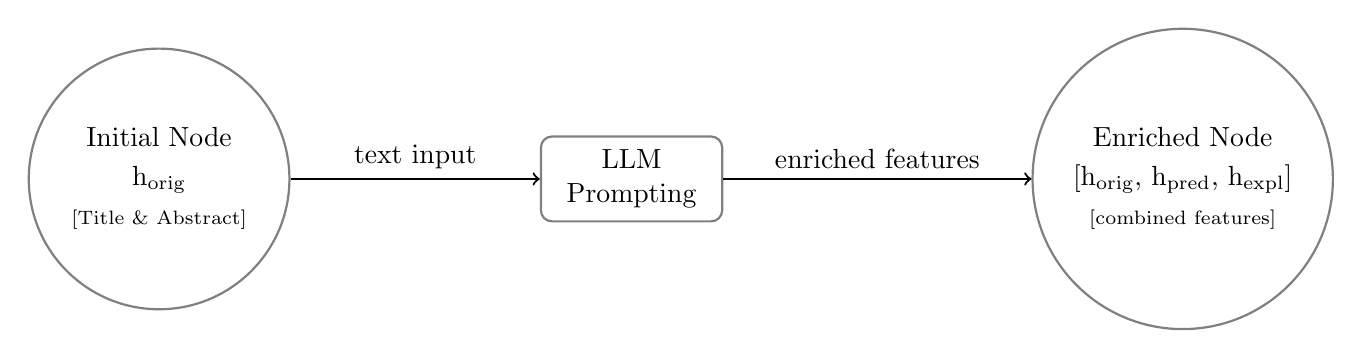
\begin{tikzpicture}[node distance=3cm,auto]
        
        % Define styles
        \tikzstyle{node} = [circle, minimum width=2.5cm, minimum height=2.5cm, draw=black!50, thick]
        \tikzstyle{process} = [rectangle, rounded corners, minimum width=2cm, minimum height=1cm, draw=black!50, thick]
        \tikzstyle{features} = [text width=2cm, align=left]
        
        % Initial node
        \node[node] (initial) {
            \begin{tabular}{c}
                Initial Node\\[2pt]
                h\textsubscript{orig}\\[2pt]
                \scriptsize{[Title \& Abstract]}
            \end{tabular}
        };
        
        % Process box
        \node[process, right of=initial, xshift=3cm] (process) {
            \begin{tabular}{c}
                LLM \\Prompting
            \end{tabular}
        };https://arxiv.org/pdf/2305.19523 was to prompt GPT 3-5 with
        the abstract and text of a document along with a questions about that document using a zero-shot approach. The
        LLM reponse then forms features which are amended to the original node representations. Issues with this approach
        
        % Enriched node
        \node[node, right of=process, xshift=4cm] (enriched) {
            \begin{tabular}{c}
                Enriched Node\\[2pt]
                [h\textsubscript{orig}, h\textsubscript{pred}, h\textsubscript{expl}]\\[2pt]
                \scriptsize{[combined features]}
            \end{tabular}
        };
        
        % Arrows
        \draw[->, thick] (initial) -- (process) node[midway, above] {text input};
        \draw[->, thick] (process) -- (enriched) node[midway, above] {enriched features};
        

        
        \end{tikzpicture}
        \caption{Node feature enrichment process using LLM and LM}
        \label{fig:llm4g}
        \end{figure}

    \subsubsection{Research Question 2}

    Proposal: Utilising more features in the encoder CAL process can improve the precision of the encoder CAL process.

    \newpage
    
    \subsection{Notes on Graph Neural Networks}


  A node is represented by a feature matrix, which contains information about the document. This \textbf{Node feature matrix}, $X$, which has the dimensions of $m$ (the number of nodes) and $n$ (the number of features). $X \in \mathbb{R}^{m \times n}$. X does not have to be a square matrix, and does not encode any information about the structure of the graph. 

  Consider 3 research papers as nodes, with features: [Author, Title Length, Abstract Length, Citation Count]
  $X = \begin{bmatrix}
  \text{"Smith"} & 82 & 500 & 45 \\
  \text{"Johnson"} & 95 & 475 & 23 \\
  \text{"Zhang"} & 67 & 612 & 89
  \end{bmatrix}$
  Where $X \in \mathbb{R}^{3 \times 4}$ represents:
  
  3 papers (rows)
  4 features per paper (columns)
  Mixed data types (categorical and numerical)

  Structural information is encoded in the \textbf{adjacency matrix}, $A$, which has the dimensions of $m$ (the number of nodes) and $m$ (the number of nodes). $A \in \mathbb{R}^{m \times m}$. A encodes information about the structure of the graph, and is used to determine relationships between nodes. Conventionally the source nodes are the rows, and the destination nodes the columns of the matrix. 1 indicates an edge between the source node $u$ and destination node $v$. Note that there is a choice to make here, with the diagonal of the matrix being 0 or 1. This choice is based on wheter you consider the source node to be connected to itself. In cases where the representation of the node is dependent on itself and adjacent nodes, the diagonal should be set to 1. In the scenario of citation networks, the diagonal should be set to 1, as a paper is likely to reference and build upon its own findings throughout. By setting the diagonal to 0, it is akin to attempting to predict the representation of the node base only on its adjacent nodes, which is not the case in citation networks. If an adjaceny metrix is symmetric around it's diagonal, then the graph is undirected, otherwise it is directed (i.e. $U$ is connected to $V$ and $V$ is conencted to $U$). In citation networks, this is not the case, as because paper A cites paper B, it does not mean the reverse is true.    

  Consider the same 3 research papers, with the following adjacency matrix:
  $A = \begin{bmatrix}
  0 & 1 & 0 \\
  0 & 0 & 1 \\
  1 & 0 & 0
  \end{bmatrix}$
  Which represents the following graph:

  \begin{center}
    \begin{tikzpicture}[
        > = {Stealth[scale=1.2]},
        vertex/.style = {circle, draw, minimum size=1.2cm, inner sep=1pt},
        ref_edge/.style = {->, thick, blue},
        label_style/.style = {font=\small}
    ]

    \node[vertex] (Smith) at (0,0) {Smith};
    \node[vertex] (Johnson) at (2,0) {Johnson};
    \node[vertex] (Zhang) at (1,2) {Zhang};

    \draw[ref_edge] (Smith) -- (Johnson);
    \draw[ref_edge] (Zhang) -- (Johnson);
    \draw[ref_edge] (Smith) -- (Zhang);
    \end{tikzpicture}
    \end{center}

    With both $X$ and $A$ defined, we can numerically represent the graph. The node feature matrix $X$ is the initial/input node features, with our goal for learning on graphs to learn node embeddings $H \in \mathbb{R}^{N\times D}$ where $D$ is a chosen hidden dimension size. 


    \subsection{Message Passing Neural Networks}

    We need an approach that can work with the graph structure, which has variable number of nodes and edge conenctions between nodes. Historically with the CNN architecture, the input size was fixed, and the network was able to learn spatial invariance through the use of convolutional filters that were invariant to the location of the feature in the input. With graph structured data, the number of nodes and connections between nodes can vary for each graph, and spatial invariance is not invariant to the location of the feature in the graph. 

    Message Passing Neural Networks (MPNNs) are a type of graph neural network that can learn spatial invariance through the use of message passing between nodes. The basic idea of MPNNs is to iteratively update node representations by passing messages between connected nodes. This process is repeated for a fixed number of iterations, or until convergence.

    The process is defined as follows:
    \begin{itemize}
        \item Message: every node decides how to send information to neighboring nodes it is conencted to by edges
        \item Aggregate: nodes recieve messages from all their neighbors, who also passed messages and decides how to combine the information from all of its neighbors. 
        \item Update: each node decies how to combine neighbourhood information with its own information and updates it embedding for the next timestep. 
    \end{itemize}

    By doing this we have nodes pass each other information and disseminate information around the graph, allowing the network to learn spatial invariance.  This can be repeated for a fixed number of iterations ($K$), with the larger the value of $K$, the more the more diffuse the information around the graph becomes.

    Each section of the MPNN process in more detail:

    \subsubsection{Message}

    The source node $U$ will pass a message $m_{uv}$ to the destination node $V$. The message depends on the GNN architecture with the easiest example message being passed being $U$ node's feature $h_u$ vector to $V$.

    \subsubsection{Aggregate}

    The destination node $V$ will recieve messages from all its neighbouring nodes, and needs to decide how to combine the information from all of its neighbours. This is typically done using a sum, average or max pooling of the messages from all neighbouring nodes. It is important that the aggregation function has to be a permutation invariant function, as the order of the messages should not affect the output. 

    This gives us a combined neighbourhood node embedding, denoted as $h_{N(V)}$, where $N(V)$ is the set of all neighbouring nodes to $V$, meaning all nodes connected to $V$ by an edge. 

    $h_{N(v)}^{k+1} = AGGREGATE({h_u^k, \forall u \in N(v)})$

    \subsubsection{Update}

    Each node updates its own embedding based on the combined neighbourhood embedding and its own embedding from the previous timestep. 

    $h_v^{k+1} = \sigma(W \cdot CONCAT(h_v^k, h_{N(v)}^{k+1}))$


    Search criteria for Graph Neural Networks and Active Learning
    ("graph neural network" OR GNN) AND ("active learning" OR "interactive learning") AND (document OR citation OR literature) AND ("relevance feedback" OR "document classification") AND ("semi-supervised" OR "partially labeled")
    Database-specific versions:

    arXiv: search within cs.LG, cs.IR, cs.CL categories
    PubMed: add "systematic review" OR "literature review" terms

    \end{document}
